\begin{figure}[t]
\centering
  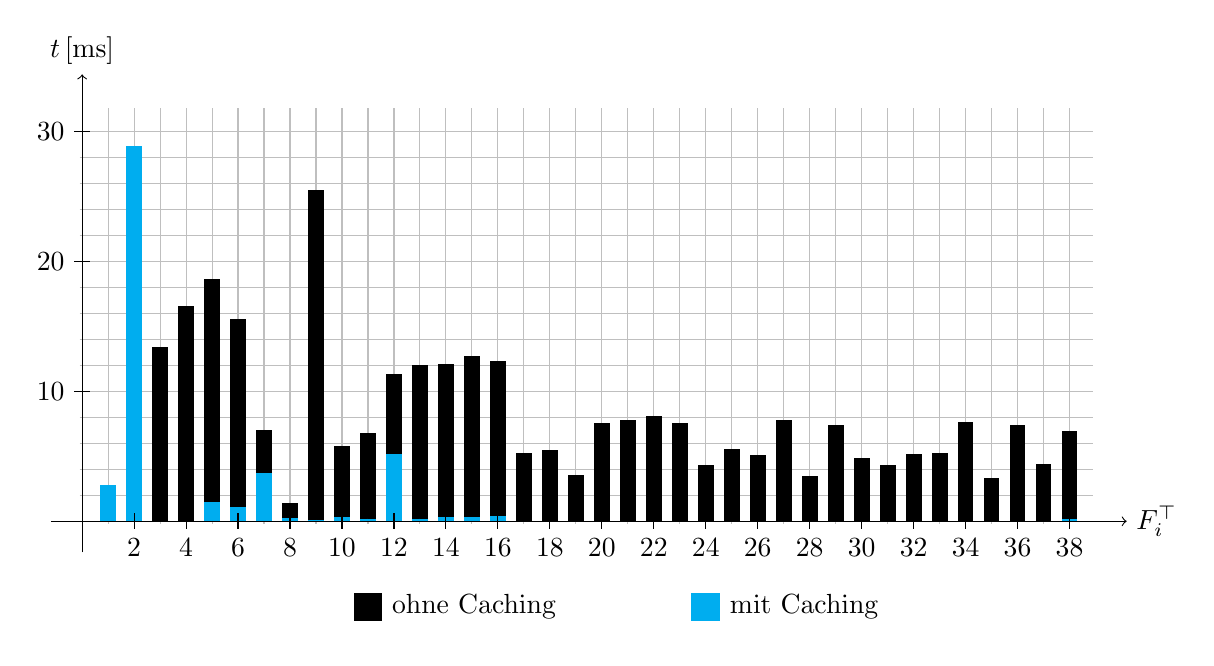
\begin{tikzpicture}[scale=0.33]
  \draw[color=lightgray] (-0.1, -0.1) grid (38.9, 15.9);
  \tikzstyle{color1}=[color=cyan, fill=cyan]

  \def\nocachevalues{{
     2.6410,
    28.5100,
    13.3869,
    16.5449,
    18.6330,
    15.5669,
     7.0220,
     1.4099,
    25.5279,
     5.8319,
     6.8040,
    11.3669,
    11.9970,
    12.0990,
    12.6920,
    12.3380,
     5.2409,
     5.4859,
     3.5239,
     7.5699,
     7.7840,
     8.0809,
     7.5949,
     4.2960,
     5.5909,
     5.1359,
     7.8219,
     3.4979,
     7.3950,
     4.8370,
     4.3480,
     5.1550,
     5.2339,
     7.6390,
     3.3230,
     7.3960,
     4.4110,
     6.9430}}

  \def\cachevalues{{
     2.7799,
    28.8550,
     0.0019,
     0.0019,
     1.4799,
     1.0950,
     3.6849,
     0.2480,
     0.0989,
     0.3180,
     0.2019,
     5.1459,
     0.1980,
     0.3459,
     0.3060,
     0.4390,
     0.0049,
     0.0020,
     0.0029,
     0.0029,
     0.0030,
     0.0300,
     0.0309,
     0.0019,
     0.0029,
     0.0039,
     0.0029,
     0.0020,
     0.0030,
     0.0019,
     0.0040,
     0.0019,
     0.0030,
     0.0029,
     0.0029,
     0.0020,
     0.0019,
     0.2120}}

  \foreach \x in {1,2,3,4,5,6,7,8,9,10,11,12,13,14,15,16,17,18,19,20,21,22,23,24,25,26,27,28,29,30,31,32,33,34,35,36,37,38}
    \pgfmathparse{\nocachevalues[\x - 1] / 2}
    \edef\nocachevalue{\pgfmathresult}
    \draw[line width=0.2cm] (\x, 0) -- (\x, \nocachevalue);

  \foreach \x in {1,2,3,4,5,6,7,8,9,10,11,12,13,14,15,16,17,18,19,20,21,22,23,24,25,26,27,28,29,30,31,32,33,34,35,36,37,38}
    \pgfmathparse{\cachevalues[\x - 1] / 2}
    \edef\cachevalue{\pgfmathresult}
    \draw[line width=0.2cm, color1] (\x, 0) -- (\x, \cachevalue);

  \draw[->] (-1.2, 0) -- (40.2, 0) node[right] {$\ma{F}^{\top}_i$};
  \draw[->] (0, -1.2) -- (0, 17.2) node[above] {$t \left[\mathrm{ms}\right]$};

  \foreach \y in {1,2,3}
    \pgfmathtruncatemacro{\label}{10 * \y}
    \draw (0.3, 5*\y) -- (-0.3, 5*\y) node[left] {\label};

  \foreach \x in {1,2,3,4,5,6,7,8,9,10,11,12,13,14,15,16,17,18,19}
    \pgfmathtruncatemacro{\label}{2 * \x}
    \draw (2*\x, 0.3) -- (2*\x, -0.3) node[below] {\label};

  \fill[white] (0, -4.5) rectangle (1, -2) node {};  % Abstand nach unten

  \tikzstyle{node}=[rectangle,draw, minimum width=10pt, minimum height=10pt, inner sep=0pt]
  \node[node, fill=black, label=right:ohne Caching] (1) at (11, -3.3) {};
  \node[node, color1,     label=right:mit Caching]  (2) at (24, -3.3) {};

\end{tikzpicture}
% Erstelle Legende.
\begin{tabular}{llllllll}
  \toprule
  1. $\gls{M}_{00}$ & 2. $\mathrm{box}$ & 3. $\mathrm{box}_x$ & 4. $\mathrm{box}_y$ & 5. $\hat{x}$ & 6. $\hat{y}$ & 7. $\mathrm{ecc}$ & 8. $\mathrm{dia}$\\
  9. $\mathrm{ext}$ & 10. $\gls{hu}_1$ & 11. $\gls{hu}_{2}$ & 12. $\gls{hu}_{3}$ & 13. $\gls{hu}_{4}$ & 14. $\gls{hu}_{5}$ & 15. $\gls{hu}_{6}$ & 16. $\gls{hu}_{7}$\\
  17. $\gls{eta}^{\prime}_{02}$ & 18. $\gls{eta}^{\prime}_{11}$ & 19. $\gls{eta}^{\prime}_{20}$ & 20. $\gls{lambda}_1$ & 21. $\gls{lambda}_2$ & 22. $\mathrm{axis}_1$ & 23. $\mathrm{axis}_2$ & 24. $\gls{mu}_{02}$\\
  25. $\gls{mu}_{03}$ & 26. $\gls{mu}_{11}$ & 27. $\gls{mu}_{12}$ & 28. $\gls{mu}_{20}$ & 29. $\gls{mu}_{21}$ & 30. $\gls{mu}_{30}$ & 31. $\gls{eta}_{02}$ & 32. $\gls{eta}_{03}$\\
  33. $\gls{eta}_{11}$ & 34. $\gls{eta}_{12}$ & 35. $\gls{eta}_{20}$ & 36. $\gls{eta}_{21}$ & 37. $\gls{eta}_{30}$ & 38. $\mathrm{ori}$ & & \\
  \bottomrule
\end{tabular}

\caption[Laufzeitverteilung einer Merkmalsextraktion]{Laufzeitverteilung einer Extraktion aller $38$ Form-Merkmale einer \gls{SLIC}-Segmentierung mit $800$ Regionen.
Die schwarzen Balken kennzeichen die einzelnen Berechnungskomplexitäten der Merkmale.
Die blauen Balken hingegen demonstrieren den Laufzeitgewinn mittels Caching bei der Berechnung aller Merkmale.
Es zeigt sich, dass bereits nach der Berechnung des zweiten Merkmals ein deutlicher Geschwindigkeitsgewinn zu vernehmen ist.}
\label{fig:merkmals_caching}
\end{figure}
